\clearpage
\section{Supplementary}

\subsection{Testing with a manufactured solution to assess accuracy.}
\label{sup:manu}

Below we will discuss the parameter identification and its sensitivity with respect to the regularization parameters, noise, number of observations and time-resolution of the forward model. 
The manufactured observations were obtained by forward computation of \eqref{Eq::PDE} with the Dirichlet boundary condition defined as 
\begin{equation}
g(t) = 0.3 +0.167t - 0.007t\sp{2} \qquad \text{ for } 0 \leq t \leq 24.
\label{EQ::DIRI}
\end{equation}
The initial condition was set to 0 everywhere, the timestep was $dt = 0.2$, and the diffusion coefficients were selected to be 
\begin{equation}
D_{\Omega_1} = 1000.0, \quad D_{\Omega_2} = 4.0, \quad D_{\Omega_3} = 8.0 
\end{equation}  

\begin{figure}
\centering
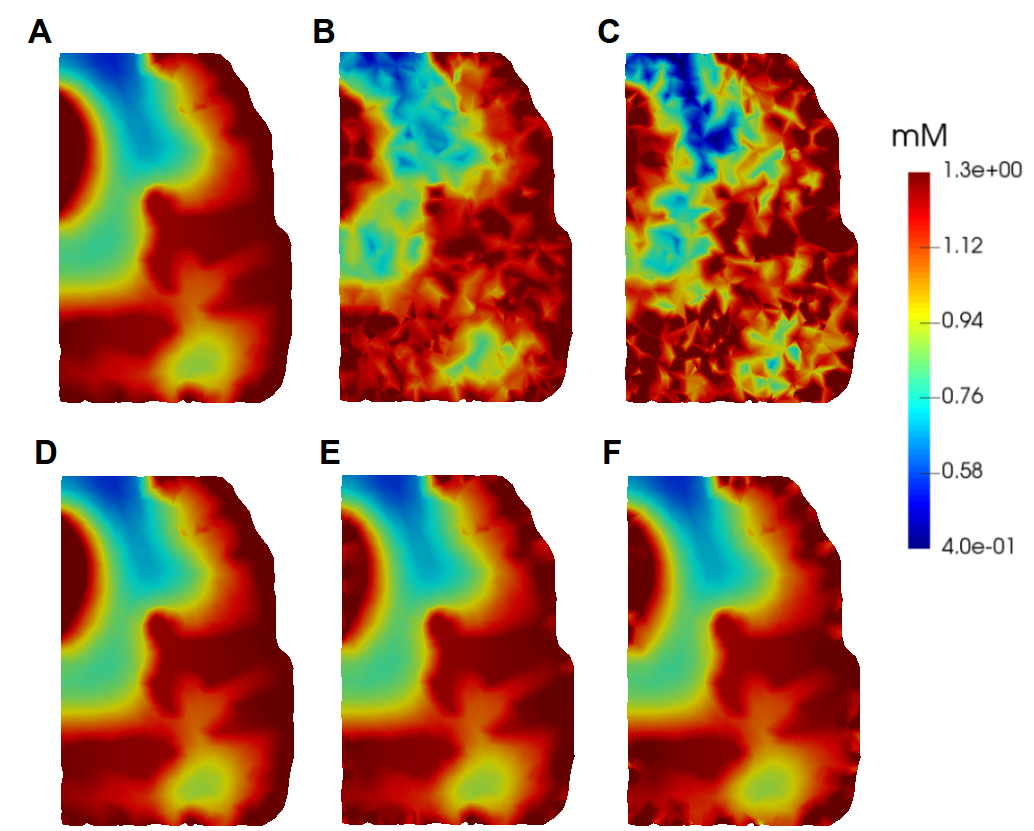
\includegraphics[scale=0.4]{../noise-12.png}  
\caption{The upper row shows the manufactured observation, A) Shows the manufactured observation at time-point 24 with no noise added. B) Shows the manufactured observation after 12 hours with noise amplitude of 0.15. C) Shows the manufactures observation after 12 hours with noise amplitude of 0.3. The lower row shows the results with optimized parameter obtained with $\alpha=0.0001$, $\beta=1.0$ and $k=20$. D) Shows the resulting state given the observation in A. E)  Shows the resulting state given the observation in B .F) Shows the resulting state given the observation in C. }
\label{12hourswithnoise}
\end{figure}





\subsection{Contrast concentration - Image Signal Relation}
Below, we briefly describe the relationship between the imaging signal 
seen in Figures~\ref{fig1} and \ref{fig2} and the underlying contrast 
concentration. We remark that we use a notation common in medical literature and here two letter symbols are common. Hence, below we will use two letter symbols such as $TE$ and $TR$ to keep the notation consistent with the presentation in \cite{GOWLAND, MPRAGE}.   
The contrast concentration $c$ causes the longitudinal(spin-lattice) relaxation time $T_{1}$ to shorten with the following relation
\begin{equation}
\frac{1}{T_{1}\sp{c}} = \frac{1}{T_{1}\sp{0}} + r_{1}c .
\label{EQ::contrast}
\end{equation}
The superscripts indicate relaxation time with contrast $T_{1}\sp{c}$ and without contrast $T_{1}\sp{0}$, and $r_1$ is the relaxivity constant for the MRI-contrast in a medium. 
The contrast observations were collected using a MRI sequence known as  Magnetization Prepared Rapid Acquisition Gradient Echo (MPRAGE) with an inversion prepared magnetization. The relation between signal and the relaxation time is non-linear, and is expressed with the following equations. The signal value $S$ for this sequence is given by
\begin{equation}
S = M_{n} \sin \theta e\sp{ - TE/T_2\sp{*} },
\label{EQ::SI_T2}
\end{equation}
with $TE$ and $\theta$ respectively denoting the echo time and the flip angle, and $M_{n}$ the magnetization for the n-echo described below. 
Also $T_2\sp{*}$ is transverse magnetization caused by a combination of spin-spin relaxation and magnetic field inhomogeneity. It is defined as 
\begin{equation}
\frac{1}{T_2\sp{*}} = \frac{1}{T_2} + \gamma \Delta B_{in} ,
\end{equation}
with $T_2$ transverse (spin-spin) relaxation time, $\gamma$ is the gyromagnetic ratio and $\Delta B_{in}$ is the magnetic field inhomogeneity across a voxel. The expression can be simplified by neglecting the $T_2$ term in the signal, since $TE <<T_2\sp{*}$ for this MRI sequence. Thus \eqref{EQ::SI_T2} becomes 
\begin{equation}
S = M_{n} \sin \theta.
\label{EQ::SI}
\end{equation}
In article \cite{GOWLAND}, the term $M_n$ is defined as the magnetization for the n-echo 
\begin{equation}
M_{n} = M_{0}  \left[ (1-\beta)\frac{(1-(\alpha \beta)\sp{n-1} }{1-\alpha\beta} + (\alpha \beta)\sp{n-1}(1-\gamma) + \gamma ( \alpha \beta)\sp{n-1} \frac{M_{e}}{M_{0}}  \right]   
\end{equation}
with 
\begin{equation}
\frac{M_{e}}{M_{0}} = - \left[ \frac{ 1 -\delta + \alpha \delta (1-\beta ) \frac{1-\alpha\beta\sp{m}}{1-\alpha \beta} + \alpha\delta(\alpha\beta)\sp{m-1} - \alpha\sp{m}\rho}{1 +\rho \alpha\sp{m} } \right].
\end{equation}
Using the following definitions
\begin{equation}
\begin{aligned}
\alpha &= \cos ( \theta ) \\
\beta  &= e\sp{- \sp{T_b}/_{T_1\sp{c}} } \\
\delta &= e\sp{- \sp{T_a}/_{T_1\sp{c}} } \\
\gamma &= e\sp{- \sp{T_w}/_{T_1\sp{c}} } \\
\rho   &= e\sp{- \sp{TR}/_{T_1\sp{c}}}  \\
T_w    &= TR - T_a -T_b(m-1)       .\\
\end{aligned}
\end{equation}
Here $T_b$ is known as the echo spacing time, $T_a$ is the inversion time, $T_w$ the time delay, $TR$ as the repetition time, $m$ is the number of echo spacings and $M_0$ is a calibration constant for the magnetization. The center echo denoted as $n=m/2$ will be the signal that we will consider when estimating MRI-contrast. Given \eqref{EQ::SI} we have that the relative signal increase can be written as 
\begin{equation}
\frac{S\sp{c}}{S\sp{0}} = \frac{ M_{n}\sp{c} \sin (\theta)}{ M_{n}\sp{0} \sin (\theta) }.
\end{equation}
We define that  
\begin{equation}
f(T_1) = M_{n}/M_{0} ,
\label{scaledmagnetization}
\end{equation}
which can be seen in Figure~\ref{figuredti}. 
This gives the following relation 
\begin{equation}
\frac{f(T_{1}\sp{c} ) }{f(T_{1}\sp{0})}  = \frac{S\sp{c}}{S\sp{0}} 
\end{equation}
The signal difference between observation times were adjusted in \cite{ringstad2018brain}. Thus we can express the change in $T_1$ due to contrast as 
\begin{equation}
f ( T_{1}\sp{c} ) = \frac{S\sp{c}}{S\sp{0}} f(T_{1}\sp{0}) 
\end{equation}
and then estimate the concentration using \eqref{EQ::contrast}. The $T_{1}\sp{0}$ values were obtained by T1-mapping of the brain using a MRI sequence known as MOLLI5(3)3 \cite{TAYLOR201667}. This takes into account patient specific characteristic, such as tissue damage. Tissue damage can be observed in the MRI due to a lower signal in the white matter compared to healthy white matter tissue, thus damaged tissue have different $T_1$ relaxation time. 
The contrast concentration was estimated in a preprocessing step, using the parameters obtained from the T1-map, MPRAGE MRI protocol \cite{ringstad2018brain} and the value for $r_1$ found in \cite{pmid16230904}. In the computation, the function \eqref{scaledmagnetization} was computed for $ T_1\in \lbrace 200, 4000 \rbrace$ creating a lookup table. The lookup table was utilized with the baseline signal increase to estimate $T_1\sp{c}$, and then the concentration was computed using \eqref{EQ::contrast}.  

\begin{figure}
\centering
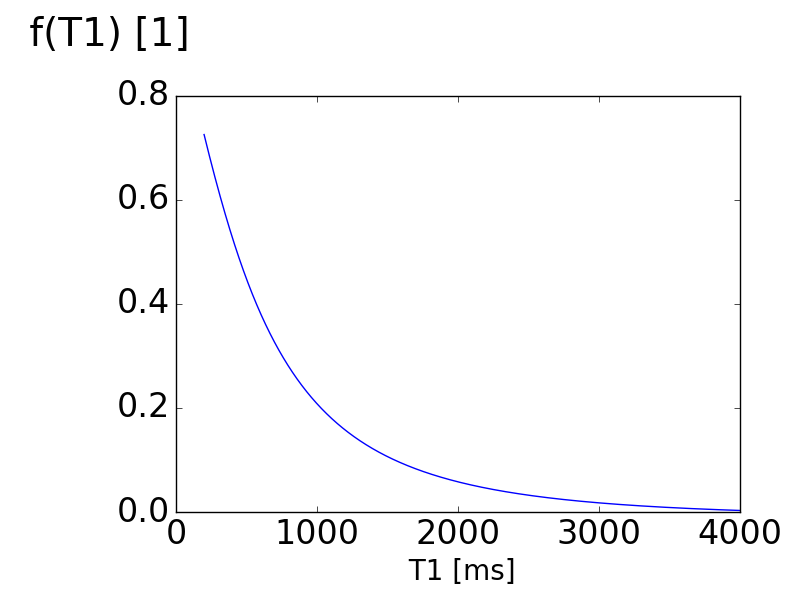
\includegraphics[width=0.70\textwidth]{../T1function.png} 
\caption{Shows the  function defined in \eqref{scaledmagnetization} where the white region indicates $T_1$ values for white matter, the grey region indicates $T_1$ values for grey matter, the blue region indicates $T_1$ values for CSF.  }
\label{figureF} 
\end{figure}


\subsection{Diffusion tensor imaging}
In addition to the T1 and T2 weighted sequences described above we have also obtained diffusion tensor imaging to assess the apparent diffusion 
coefficients on short time-scales. Images are shown in Figure~\ref{figuredti} where the largest diffusion coefficient (shown in 
red in the middle figure) is shown to be around $1.0\mathrm{e}{-3}  \mathrm{mm^2/s}$. We remark that we have not included possible anisotropy, shown in 
the right-most image in Figure~\ref{figuredti} and that these images show the apparent diffusion coefficient for free water molecules (18 Da).      
The diffusivity of the Gadovist (600 Da) \cite{MGadobutrol} was estimated to be similar to the diffusion coefficient of Gd-DPTA (550 Da) \cite{MGgDPTA}. This is due to the fact that both molecules have similar mass, and based on Stoke-Einstein equation should also have similar diffusion coefficients. The free diffusion coefficient for Gd-DPTA was estimated in \citet{GdDPTA-DIFFUSION} to be $3.8\mathrm{e}{-4}\mathrm{mm\sp{2}/s}$.
The fractional anisotropy is defined as 
\begin{equation}
FA\sp{2} =  \frac{3}{2} \frac{ (\lambda_1 - MD )\sp{2} +(\lambda_2 - MD )\sp{2} +(\lambda_3 - MD )\sp{2}}{\lambda\sp{2}_1 + \lambda\sp{2}_2  +\lambda\sp{2}_3 },
\end{equation}
with the mean diffusivity $MD$ defined as 
\begin{equation}
MD = \frac{\lambda_1 +\lambda_2 +\lambda_3 }{3}.
\end{equation}
In these equations $\lambda_i$ denotes the eigenvalues of the diffusion tensor.
\begin{figure}
\centering
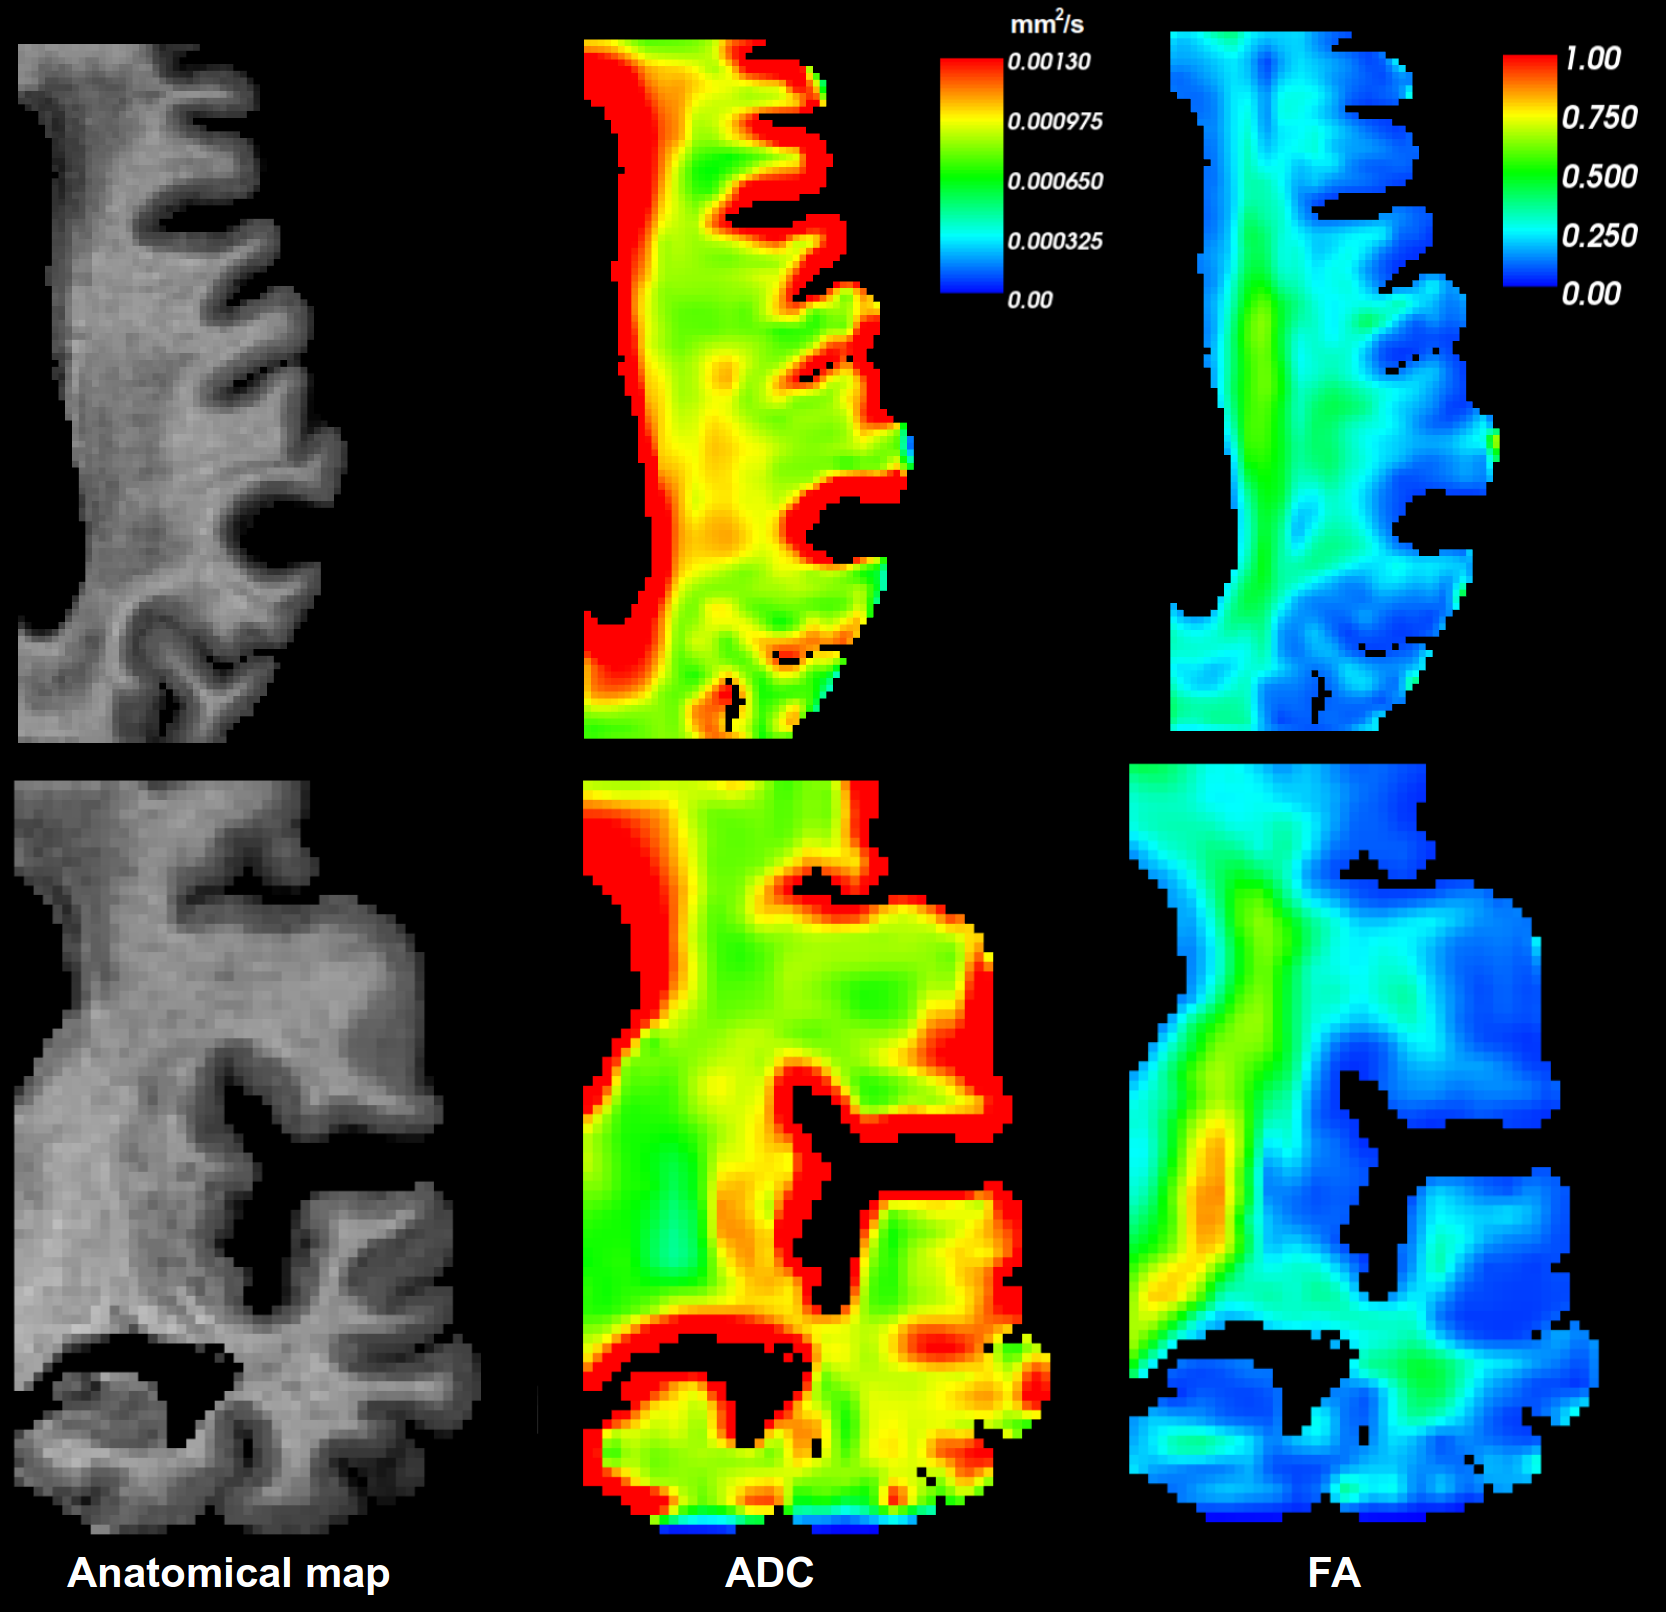
\includegraphics[width=0.75\textwidth]{../DTI-zoom.png} 
\caption{The left panel shows the anatomical map. The middle panel shows the apparent diffusion coefficients (ADC) obtained from DTI. The right panel shows the computed fractional anisotropy (FA) from the DTI.}
\label{figuredti} 
\end{figure}


\begin{figure}
\centering
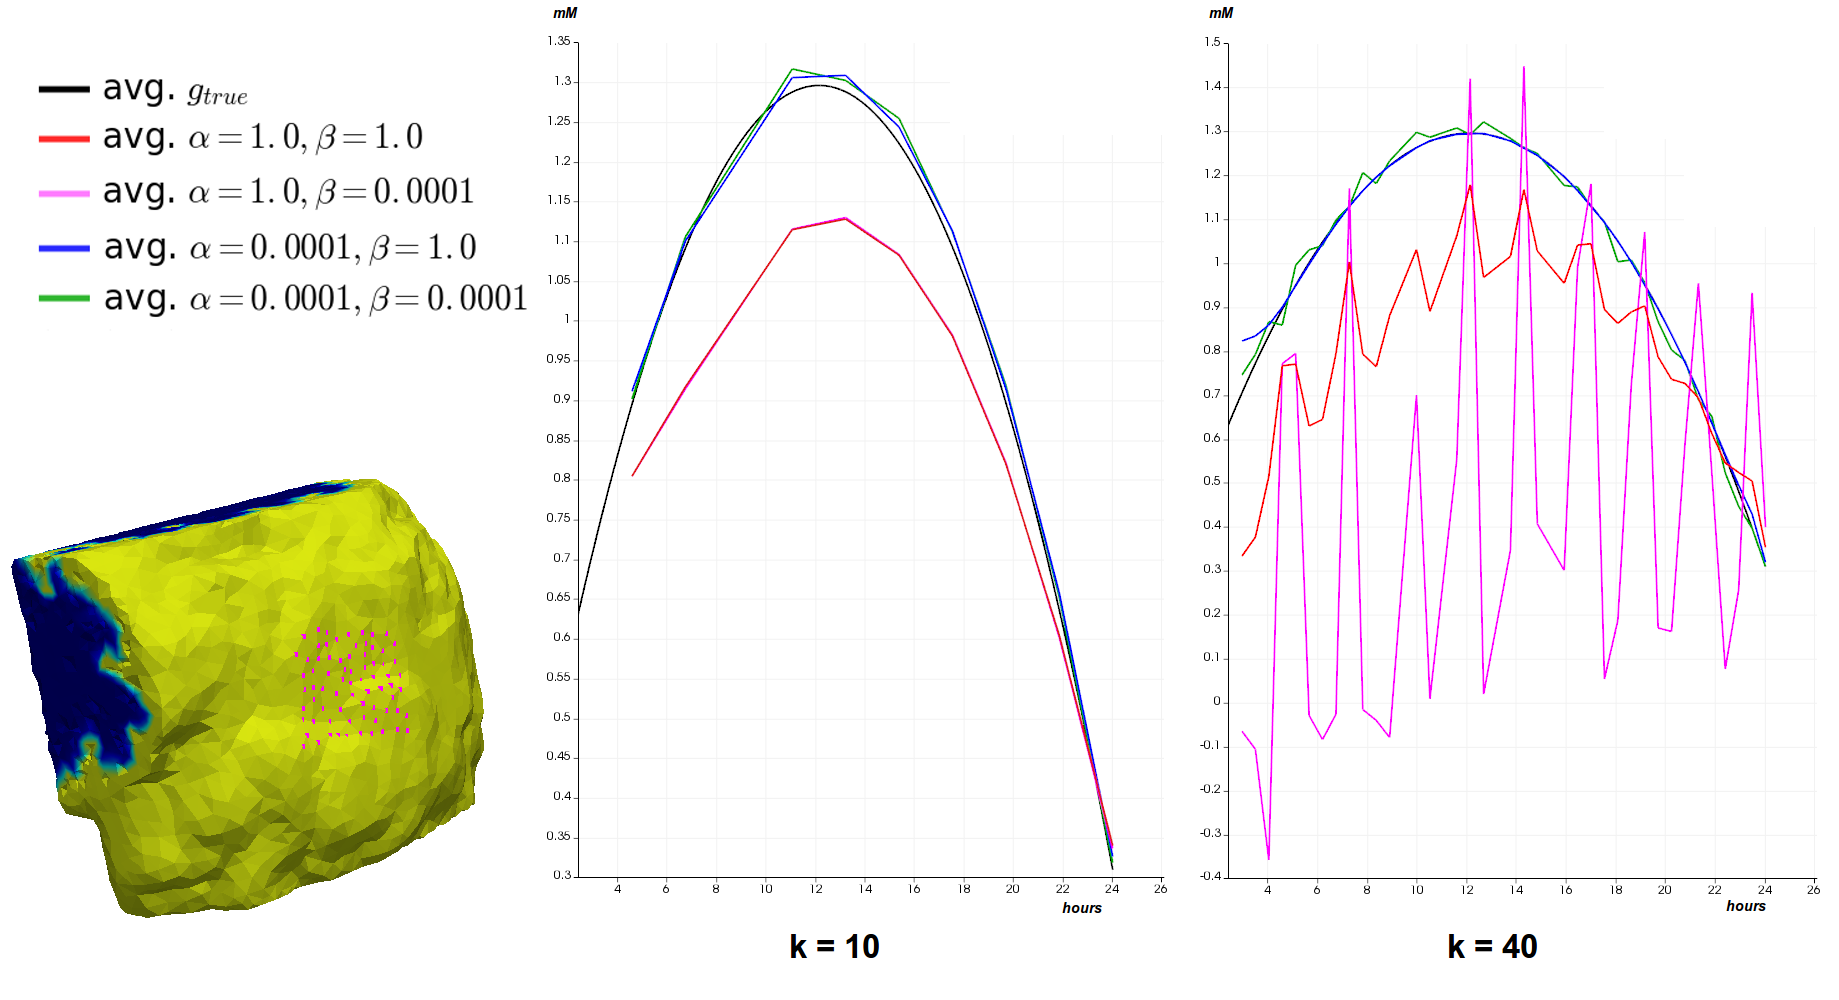
\includegraphics[scale=0.21]{../boundary_control.png}  
\caption{ Displays plots over time for a selection of points at the boundary of $\Omega_1$ with different regularization parameters and number of timesteps $k$. The left panel shows the legend for the plot over time, together with the selection of points. The middle panel shows the average boundary value $g$ for different regularization parameter with $k=10$. The right panel shows the average boundary value $g$ for different regularization parameter with $k=40$.  }
\label{boundarycontrol}
\end{figure}


\begin{figure}
\centering
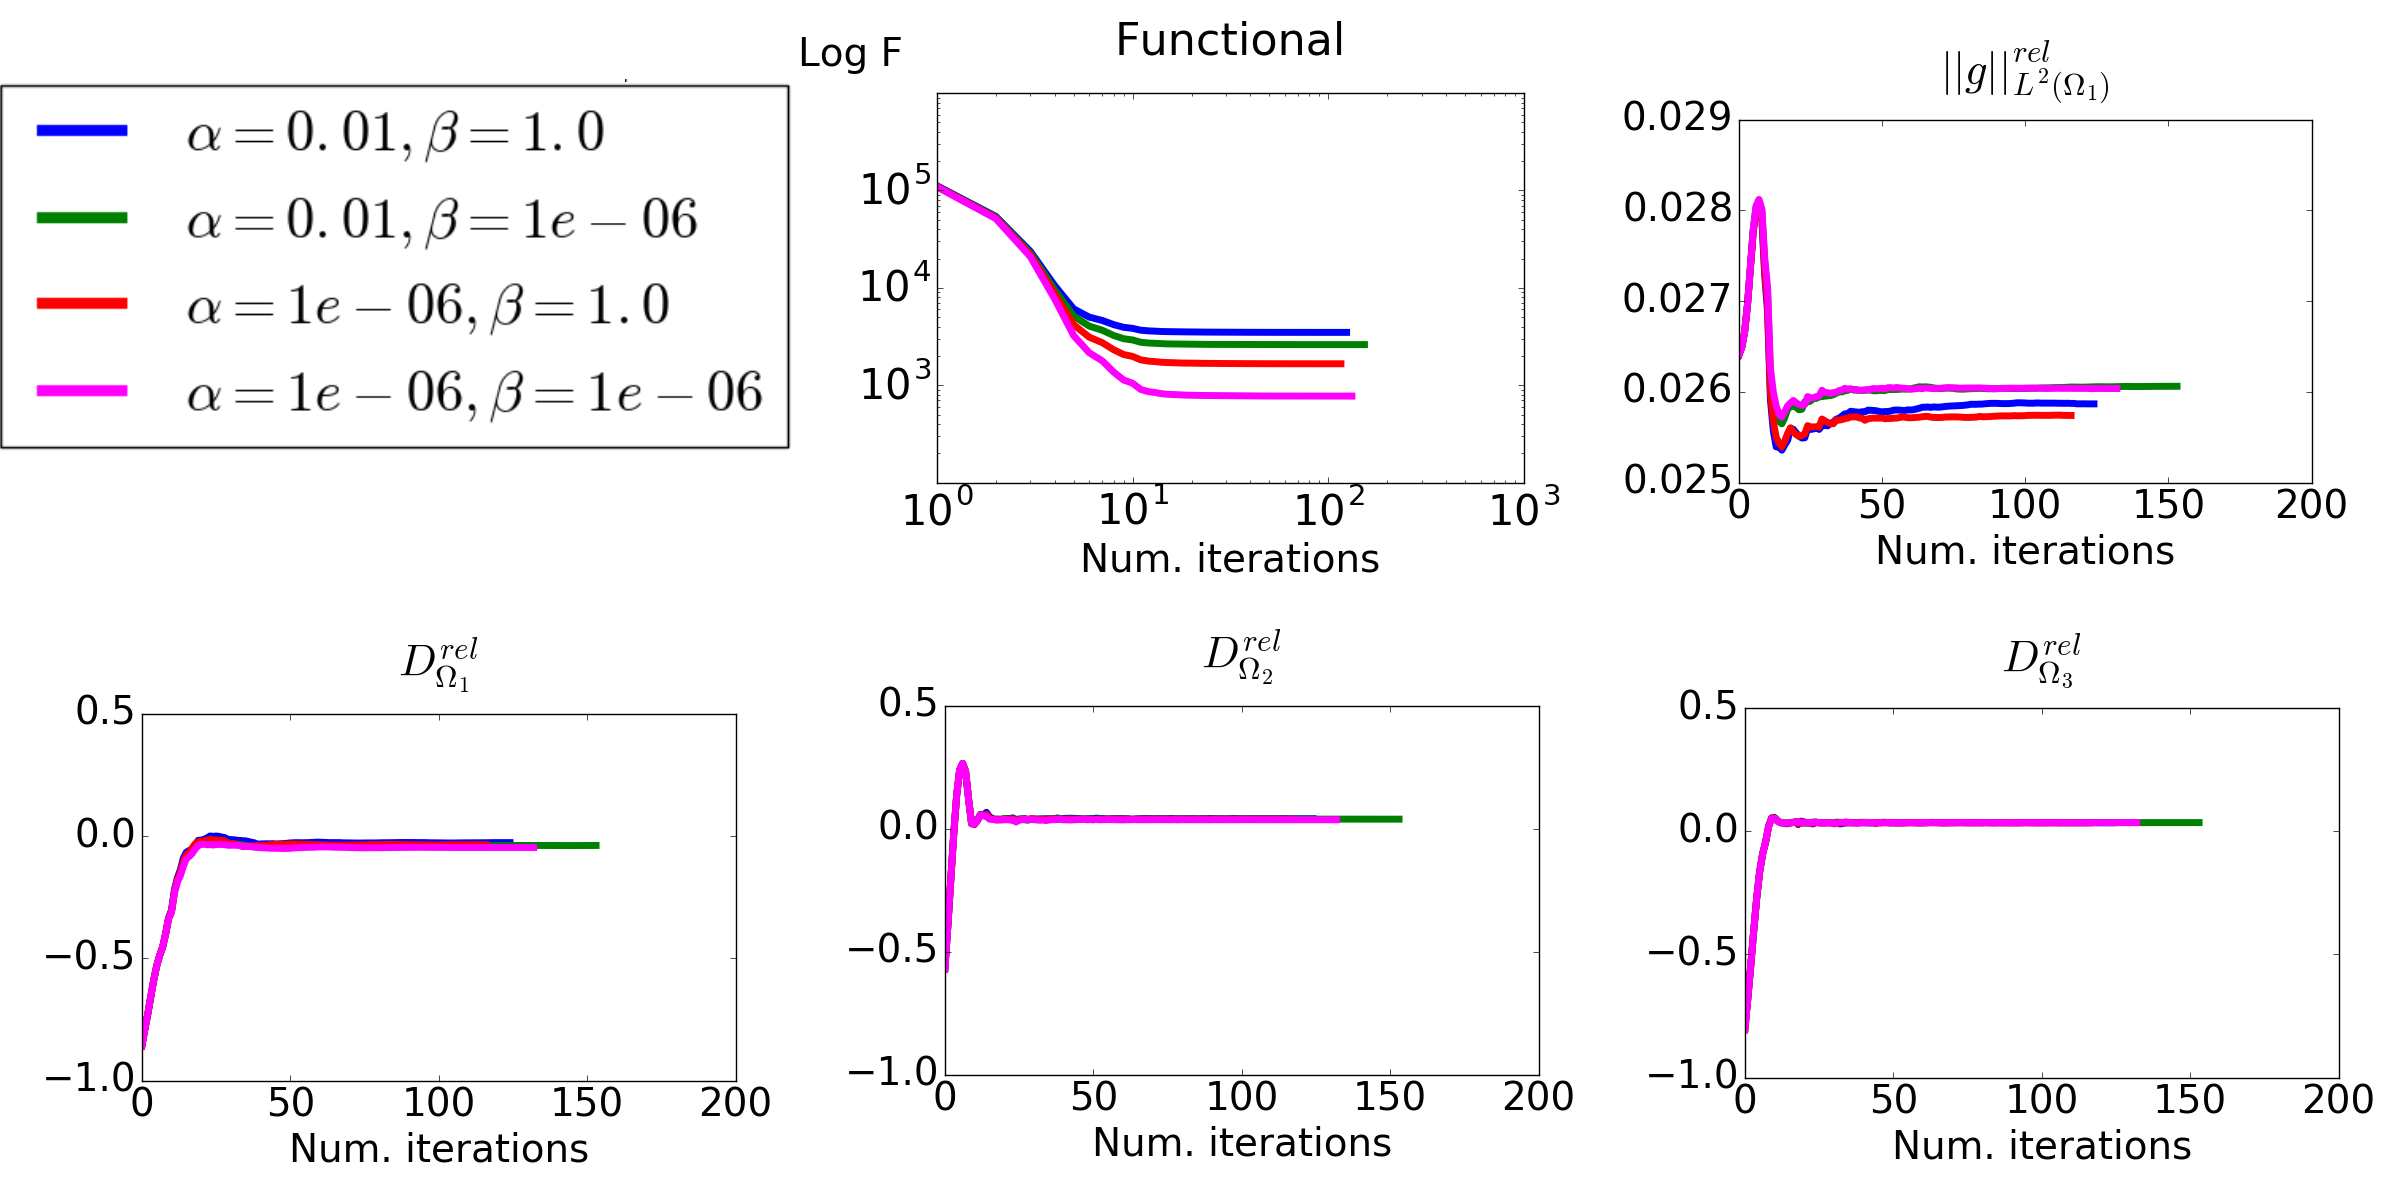
\includegraphics[scale=0.18]{../Convergence-plot.png}   
\caption{Convergence plots of the diffusion coefficients, boundary conditions and functional with respect to different $\alpha$ and $\beta$ values. } 
\label{convergence}
\end{figure}




